\chapter{Experimentación}


% ------------------------------------------------------------------------------------------------------------
% ------------------------------------------------------------------------------------------------------------

\section{Protocolo de validación experimental}

Como se ha comentado anteriormente, se han proporcionado los datos ya dividos en conjunto de entrenamiento
(\textit{train}) y de test, para evitar problemas asociados al \textit{data snooping}. 
\footnote{
    El \textbf{\textit{data snooping}} ocurre cuando información del conjunto de test se filtra, directa 
    o indirectamente, en el proceso de entrenamiento del modelo, lo que puede llevar a una sobreestimación del 
    rendimiento y a modelos que generalizan pobremente en datos nuevos
}.
Al proporcionar las particiones predefinidas, se garantiza que no haya contaminación entre los datos de 
entrenamiento y test, manteniendo así la validez de las métricas obtenidas en el test. 

Sin embargo, si se optimizan los parámetros del modelo durante el entrenamiento sin disponer de un conjunto 
independiente para evaluar su rendimiento, se corre el riesgo de sobreajustarse a los datos de entrenamiento.
Es por ello que, además del conjunto de entrenamiento y test, es esencial tener un \textbf{conjunto de 
validación} independiente que permita evaluar el modelo durante su desarrollo, ajustar hiperparámetros y 
comparar diferentes configuraciones sin contaminar la evaluación final en el conjunto de test.
Se consideró realizar validación cruzada (\textit{cross-validation}), pero debido al elevado coste 
computacional que implica, los resultados satisfactorios obtenidos mediante una simple partición de los datos 
(\textit{train/validation split}), se decidió prescindir de su aplicación.

En la Figura \ref{fig:data_split_base} podemos ver la división del \textit{dataset} planteada. Cabe comentar
que la división se ha realizado de forma estratificada en base a la edad y el sexo
\footnote{La estratificación se realizó en intervalos de medio año de edad y por sexo; por ejemplo, una 
instancia con edad 17.7 y sexo masculino se etiquetó como ``17.5\_M''.}.

\begin{figure}[h]
    \centering
    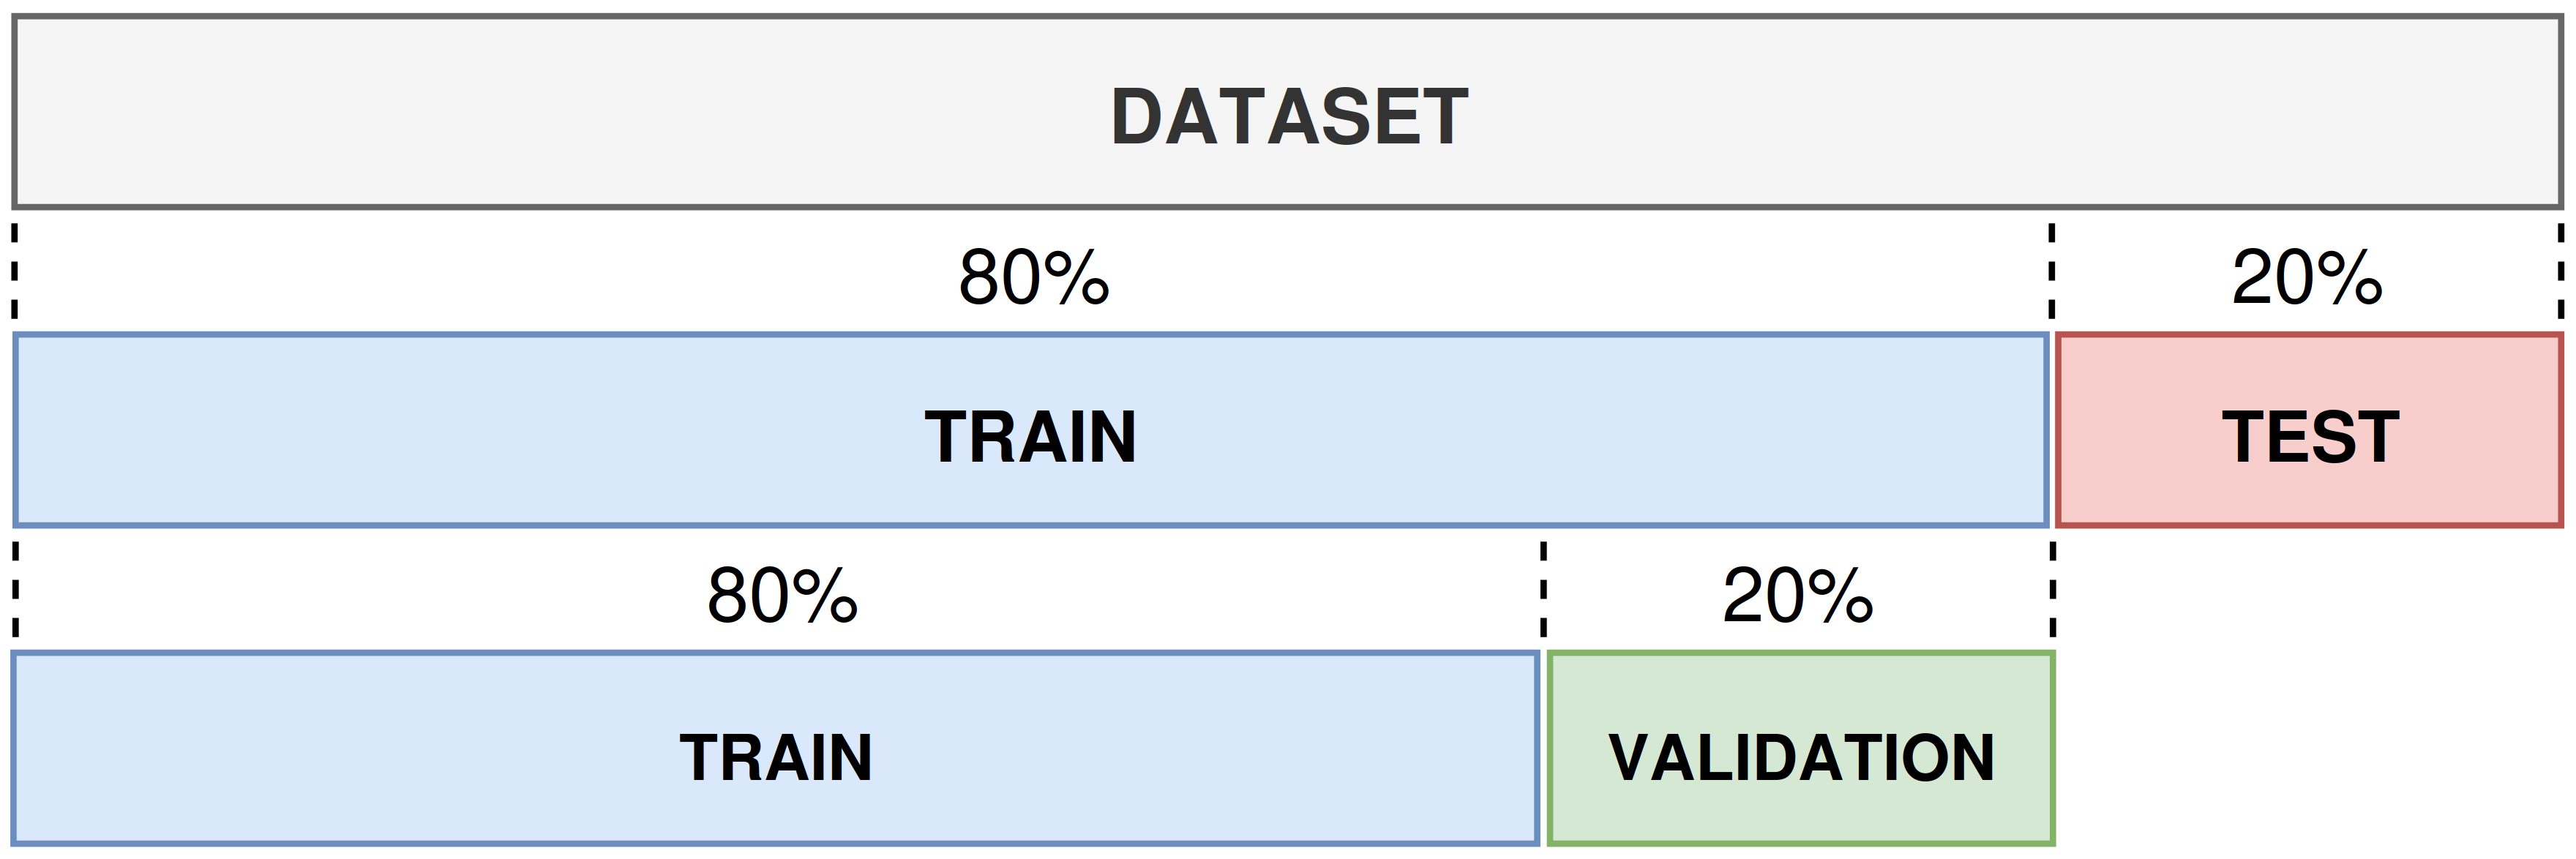
\includegraphics[width=0.8\textwidth]{capitulos/cap_04/imagenes/data_split_base.png}
    \caption[
        Diagrama de división del \textit{dataset} en \textit{train}, \textit{validation} y \textit{test}.
    ]{
        Diagrama de división del \textit{dataset} en \textit{train}, \textit{validation} y \textit{test}. 
        Elaboración propia.
    } 
    \label{fig:data_split_base}
\end{figure}

Es importante destacar que esta división se mantiene constante en todos los experimentos y para todos los 
problemas planteados, asegurando que las mismas instancias permanezcan en los mismos subconjuntos.
Esto permite garantizar que ningún modelo preentrenado reutilice datos previamente utilizados en etapas de 
validación o calibración, algo especialmente relevante dado que los problemas abordados están jerárquicamente 
relacionados (la clasificación de sexo y mayoría de edad se deriva directamente de la clasificación de 
mayoría de edad, que a su vez se deriva de la estimación de edad).

Sin embargo, al emplear métodos de calibración o predicción conformal, si usamos los mismos datos de 
entrenamiento para la calibración, 
las probabilidades o intervalos de predicción tenderán a ser optimistas, pues el modelo ha sido entrenado
con esos datos \cite{niculescu2005}. Por tanto, para evitar el sobreajuste y garantizar validez estadística 
se requiere de un subconjunto de datos adicional: el \textbf{conjunto de calibración}. Se ha escogido destinar
el  20\% de los ejemplos de entrenamiento para calibración, basándose en los resultados empíricos de 
\cite{sesia2020} (que recomienda dedicar entre un 10\% y 30\% de datos de entrenamiento a calibración), 
tal y como se muestra en la Figura \ref{fig:data_split_conformal}.

\begin{figure}[h]
    \centering
    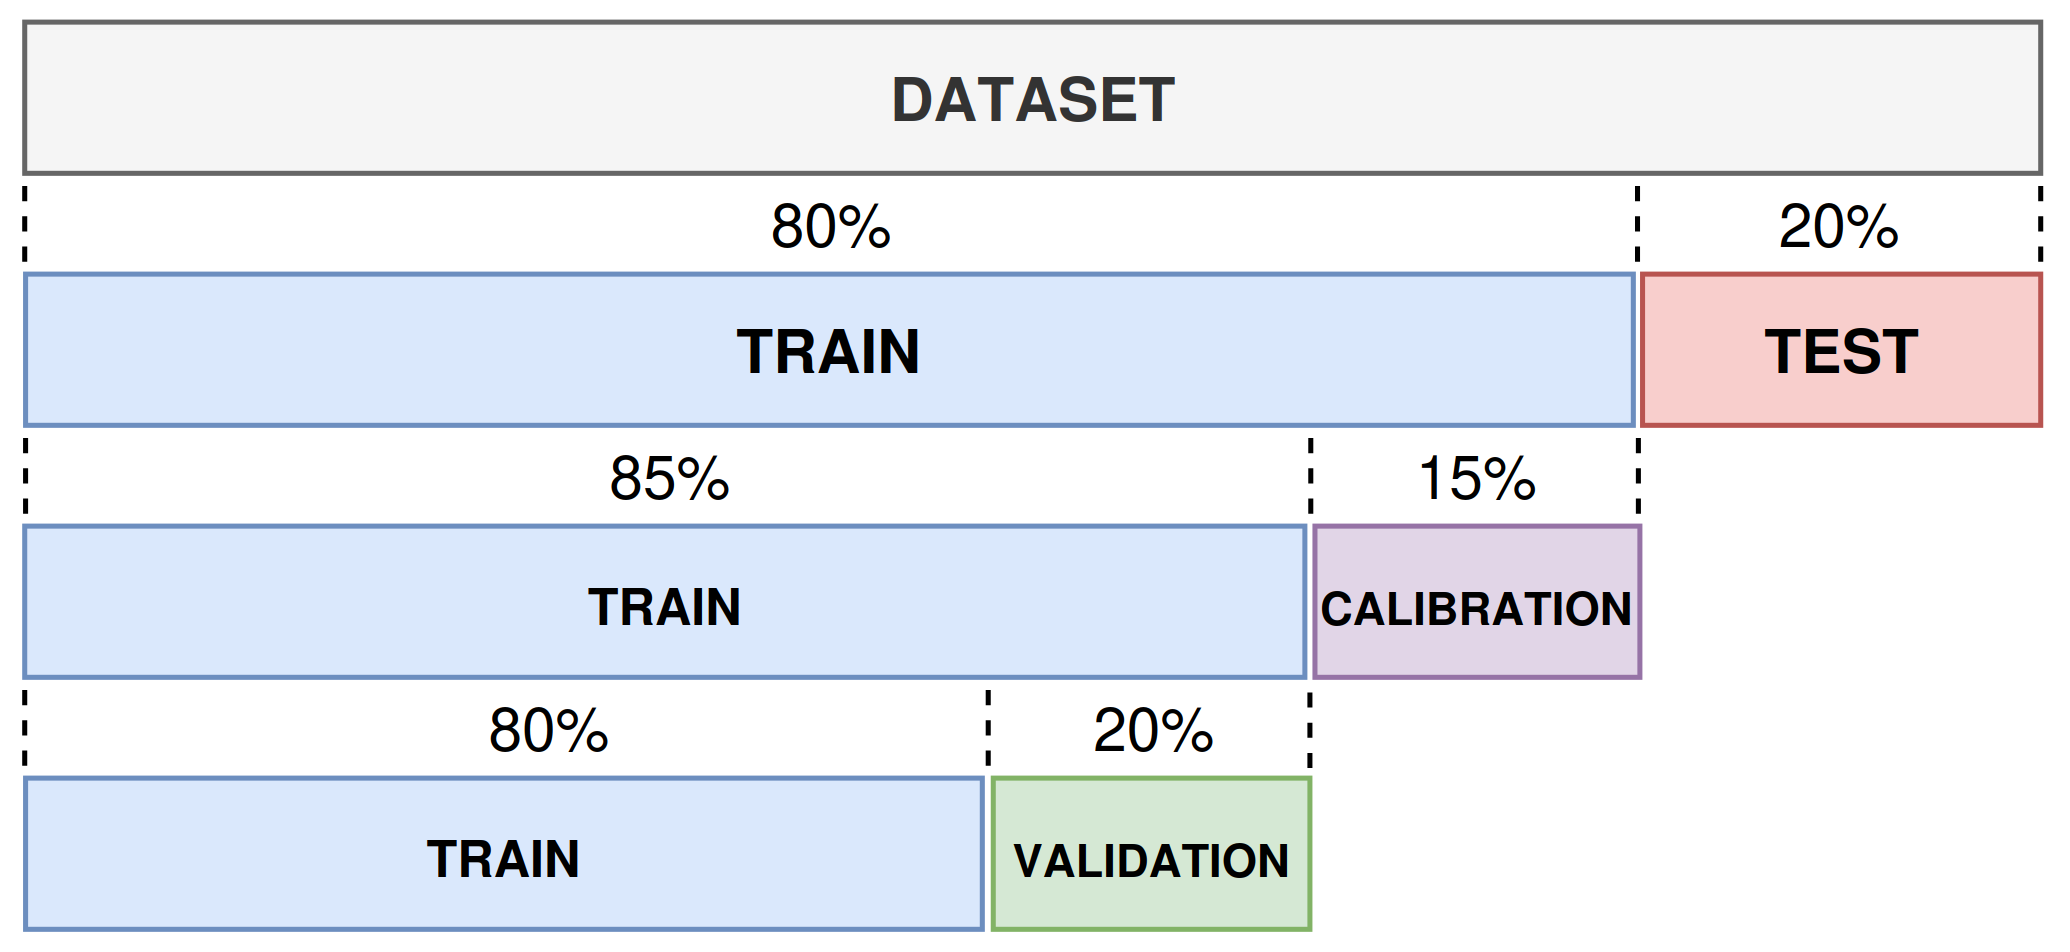
\includegraphics[width=0.8\textwidth]{capitulos/cap_04/imagenes/data_split_conformal.png}
    \caption[
        Diagrama de división del \textit{dataset} en \textit{train}, \textit{validation}, \textit{calibration} 
        y \textit{test}.
    ]{
        Diagrama de división del \textit{dataset} en \textit{train}, \textit{validation}, \textit{calibration}
        y \textit{test}. Elaboración propia.
    } 
    \label{fig:data_split_conformal}
\end{figure}

Para una comparativa más justa entre los métodos que usan CP y los que no, se utilizará la siguiente 
estrategia: los métodos que no emplean CP seguirán el esquema tradicional de división de datos (en 
entrenamiento, validación y test), mientras que los métodos basados en CP incorporarán además un conjunto 
de calibración independiente. Esta diferencia en el diseño experimental nos permitirá cuantificar cómo afecta 
a la capacidad predictiva de los modelos el hecho de reservar parte de los datos para el proceso de 
calibración.






% El objetivo del ML es establecer una hipótesis que se ajuste de forma óptima a los ejemplos futuros. Para 
% ello, suponemos que los ejemplos futuros mostrarán un comportamiento similar a los pasados. Bajo este 
% supuesto, el ajuste óptimo de un modelo es, por tanto, la hipótesis que minimiza la tasa de error del 
% problema \cite{rusell2021}. 

% Pero medir el error del modelo sobre los mismos datos empleados en el entrenamiento suele sesgar el resultado, 
% ya que el modelo puede estar sobreajustado (\textit{overfitting}) a los datos de entrenamiento, capturando no 
% solo el patrón subyacente, sino también el ruido o las peculiaridades específicas de ese conjunto de datos.
% Para evitar esto, es fundamental evaluar el modelo en un conjunto de datos de prueba independiente, que simule 
% cómo se comportaría con ejemplos futuros no vistos durante el entrenamiento. Por este motivo, es común dividir 
% los datos disponibles en dos conjuntos distintos: el \textbf{conjunto de entrenamiento (\textit{training 
% set})} y \textbf{conjunto test (\textit{test set})}.

% Aun así, incluso con esta división de conjuntos, puede persistir el riesgo de sobreajuste si se realizan 
% múltiples ajustes y selecciones de hiperparámetros basados en el rendimiento en el conjunto test.
% Esto se debe a que, indirectamente, el modelo podría estar ``aprendiendo'' características específicas del 
% conjunto de prueba, comprometiendo su capacidad de generalización. Para abordar este problema, se introduce 
% un tercer subconjunto: el \textbf{conjunto de validación}. Este conjunto se utiliza para evaluar y ajustar 
% los hiperparámetros del modelo durante el desarrollo, reservando el conjunto test únicamente para la 
% evaluación final.

% Además, técnicas como la \textbf{validación cruzada (\textit{cross-validation})} son ampliamente utilizadas 
% para maximizar el uso de los datos disponibles, especialmente en conjuntos pequeños. En lugar de una única 
% división entrenamiento-validación, este método:

% \begin{enumerate}
%     \item Divide los datos en $k$ particiones (\textit{folds}) (véase la Figura \ref{fig:CVDiagram}).
%     \item En cada iteración, usa $k-1$ particiones para entrenamiento y la restante para validación, rotando
%     sistemáticamente la partición de validación hasta que cada una de las $k$ particiones haya sido utilizada 
%     exactamente una vez como conjunto de validación. 
%     \item Promedia los resultados de todas las iteraciones para obtener una métrica robusta.
% \end{enumerate}

% El modelo final se entrena con todos los datos de entrenamiento (incluyendo los usados en validación durante 
% el ajuste). Si bien esta técnica proporciona estimaciones más confiables, su costo computacional es 
% significativo, ya que requiere entrenar el modelo $k+1$ veces ($k$ iteraciones de validación más el 
% entrenamiento final), lo que puede ser prohibitivo para modelos complejos, como redes neuronales profundas.

% \begin{figure}[h]
%     \centering
%     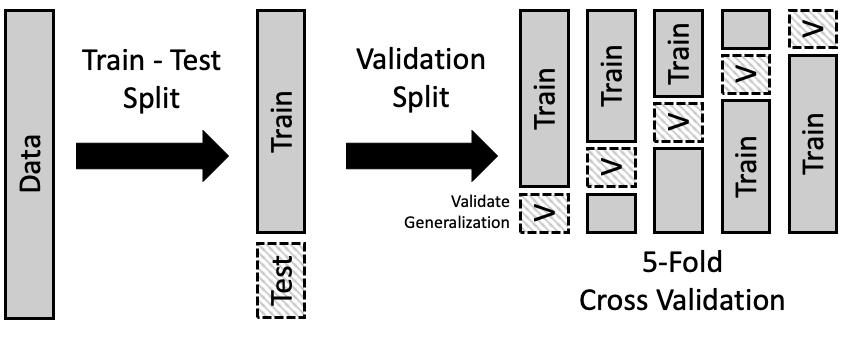
\includegraphics[width=0.95\textwidth]{capitulos/cap_05/imagenes/CVDiagram.png}
%     \caption{
%         Diagrama de división del dataset para la validación cruzada. 
%         Recuperado de \cite{lau2023crossvalidation}.
%     } 
%     \label{fig:CVDiagram}
% \end{figure}




% ------------------------------------------------------------------------------------------------------------
% ------------------------------------------------------------------------------------------------------------

\section{Experimentos propuestos}

% ------------------------------------------------------------------------------------------------------------

\subsection{Experimentos para la estimación de edad}

Se plantea una comparativa entre diversos métodos de predicción para el problema de AE. 
Todos los métodos presentan tanto predicción puntual como interválica. De esta forma queremos evaluar
tanto su utilidad tradicional para estimar el valor más probable como su capacidad para proporcionar
intervalos de confianza fiables que capturen la incertidumbre predictiva y sean computacionalmente eficientes.

Los métodos seleccionados abarcan tanto aproximaciones clásicas como técnicas modernas de conformal prediction,
lo que nos permitirá analizar:
\begin{itemize}
    \item La precisión en la estimación puntual.
    \item La validez y eficacia de los intervalos de predicción.
    \item El coste computacional asociado a cada aproximación.
\end{itemize}

El objetivo es alcanzar el 95\% de confianza en las predicciones interválicas, que es la cifra de confianza
generalmente empleada en AF. 
Los métodos propuestos son los siguientes: 

\begin{itemize}
    \item \textbf{Método `base'}: Se trata de un modelo de regresión puntual sin técnicas de CP. La predicción 
    interválica se construirá con la predicción puntual +/- 2 veces el error absoluto medio obtenido en el
    conjunto de validación, que es una aproximación heurística común para construir intervalos de predicción 
    sin distribución de errores.
    Este método sirve como \textit{baseline} para comparar la mejora que aportan las técnicas más 
    sofisticadas.

    \item \textbf{Método `ICP'}: Implementa el método ICP, mediante el cual se ...
    
    \item \textbf{Método `QR'}: Este modelo implementa QR. Utiliza tres cuantiles 
    $$
    [0.5, \alpha/2, 1-\alpha/2]
    $$ 
    para predecir la predicción puntual, límite inferior y límite superior, respectivamente.

    \item \textbf{Método `CQR'}: Este modelo implement

\end{itemize} 

Para cada método se entrenarán 10 modelos independientes desde cero, con el objetivo de capturar la 
variabilidad inherente al proceso de entrenamiento. Esto permite una comparación más robusta del rendimiento 
entre métodos. Además, se busca mantener condiciones de entrenamiento lo más reproducibles posible, a pesar 
de que cada técnica pueda utilizar diferentes funciones de pérdida. Cabe destacar que los métodos con y sin 
CP se entrenan por separado, ya que emplean divisiones distintas del conjunto de datos: mientras los métodos 
sin CP aprovechan un mayor volumen de datos de entrenamiento, los métodos con CP requieren reservar una parte 
del conjunto para calibración.

% ------------------------------------------------------------------------------------------------------------

\subsection{Experimentos para la estimación de mayoría de edad}

Todos los métodos propuestos para el problema de AAM presentan una predicción puntual ---de una sola 
etiqueta---, además de un conjunto de predicción, formado por una o más etiquetas. 

Los métodos propuestos son:

\begin{itemize}

\item \textbf{Método `base'}: Se trata del modelo de clasificación de una sola etiqueta sin uso de técnicas de 
CP. El conjunto de predicción se considerará aquel formado exclusivamente por la clase más probable. 
El entrenamiento de este modelo partirá de un modelo `base' ya entrenado para el problema de AE, al cual se 
realizará un \textit{fine-tuning} de la cabecera.  
Este método sirve de \textit{baseline} para comparar con el resto. 

\item \textbf{Método `LAC'}: Este método implementa la técnica LAC para CP. 
El entrenamiento del modelo partirá de un modelo ICP ya entrenado para regresión.

\item \textbf{Método `MCM'}: Este método implementa la técnica MCM para CP. 
El modelo será exactamente el mismo que el de LAC. Solo cambiará la calibración e inferencia conformal. 

\end{itemize} 

No se han implementado los métodos APS y RAPS, puesto que no son aplicables directamente al caso de 
clasificación binaria.

A diferencia de lo que ocurría en la regresión, las etiquetas predichas aquí darán los mismos resultados en 
todos los métodos CP, ya que usarán el mismo modelo con la misma salida puntual. 
Por tanto, el análisis se centrará principalmente en evaluar la validez de la cobertura y la eficiencia del 
conjunto de predicción generado por cada técnica de CP, considerando métricas como la tasa de cobertura 
empírica y el tamaño promedio del conjunto predicho.


% ------------------------------------------------------------------------------------------------------------

\subsection{Experimentos para la clasificación combinada de mayoría de edad y sexo}

Al igual que en el problema de AAM, para el problema de AMSC se ha seguido la misma lógica de evaluación, 
aplicando tanto predicción puntual como técnicas de CP para obtener conjuntos de predicción. 
\todo{No me gusta mucho usar estas siglas en el texto, no sé si debería directamente eliminarlas del trabajo
o solo dejarlas para usar en los resultados (para tablas y gráficos, donde no cabe mucho texto)}

En este caso, se ha empleado la técnica de calibración de probabilidades \textit{Platt Scaling} para ajustar 
las salidas del modelo de clasificación multiclase, con el objetivo de mejorar la calidad de las 
probabilidades utilizadas durante la fase de inferencia conformal. Esta calibración probabilística se 
realiza antes de aplicar los métodos de CP.
Se ha optado por utilizar el conjunto de validación para llevar a cabo dicha calibración de probabilidades, 
dado que, aunque no es el enfoque más riguroso ---ya que lo ideal sería dividir el conjunto de calibración en 
dos subconjuntos independientes, uno para la calibración de probabilidades y otro para la calibración 
conformal--- esta estrategia mostró buenos resultados en la práctica. Esto se debe a que el conjunto de 
validación empleado era suficientemente representativo y permitió obtener probabilidades calibradas de manera 
adecuada. Esta calibración probabilística no afecta a la variabilidad entre modelos con los mismos pesos, 
dado que el algoritmo es determinístico y produce resultados consistentes para un mismo conjunto de datos y 
parámetros. 

Partiendo de esto, los métodos propuestos son:

\begin{itemize}

\item \textbf{Método `base'}: Al igual que en AMM, funciona como un clasificador normal sin métodos de CP, y
se usa de \textit{baseline} para comparar con el resto.
El entrenamiento de este modelo partirá de un modelo `base' ya entrenado para el problema de AMM.

\item \textbf{Método `LAC'}: Este método implementa la técnica LAC para CP. 
El entrenamiento de este modelo partirá del modelo `LAC' ya entrenado para el problema de AMM.

\item \textbf{Método `MCM'}: Este método implementa la técnica MCM para CP. 
El modelo será exactamente el mismo que el de LAC para este mismo problema. 

\item \textbf{Método `APS'}: Este método implementa la técnica APS para CP. 
El modelo será exactamente el mismo que el de LAC para este mismo problema.

\item \textbf{Método `RAPS'}: Este método implementa la técnica RAPS para CP. 
El modelo será exactamente el mismo que el de LAC para este mismo problema. 

\end{itemize} 


% ------------------------------------------------------------------------------------------------------------
% ------------------------------------------------------------------------------------------------------------

\section{Entrenamiento de los modelos}

\subsection{Preparación de los datos de entrenamiento}

Dado que las imágenes del conjunto de datos disponible son significativamente más anchas que altas, se ha 
optado por adaptar su tamaño a 448x224.  
Se ha establecido un tamaño de \textit{batch} de 32, tras encontrar preeliminarmente un equilibrio entre 
regularización y buen ritmo de aprendizaje. 
Y también se ha realizado \textit{data augmentation} en el conjunto de entrenamiento, introduciendo 
transformaciones aleatorias en cada época para simular condiciones de posicionamiento del paciente y de la 
máquina e iluminación ligeramente variables: 
\begin{itemize}
    \item volteo horizontal en la mitad de las imágenes,
    \item rotación entre -3 y 3 grados,
    \item traslaciones de hasta el 2\%,
    \item escalado entre el 95 y 105\%, y
    \item cambios de brillo y contraste entre 80 y 120\%. 
\end{itemize}

% ------------------------------------------------------------------------------------------------------------

\subsection{Adaptación de la red para la estimación de edad}

Como se venía anticipando en el anterior capítulo, adaptaremos la arquitectura del modelo ResNeXt50 para el 
problema de regresión. El tamaño de las imágenes de entrada no modifica la arquitectura del modelo, pues el 
extractor de características conserva la dimensionalidad relativa a través de sus bloques convolucionales, 
si bien todas las imágenes las hemos adaptado al tamaño 448x224 para garantizar una entrada uniforme.
Sustituiremos la última capa del modelo por un \textit{adaptive average pooling}, que permite reducir la 
dimensionalidad espacial de forma flexible independientemente del tamaño exacto de entrada. A continuación, 
este tensor de características se aplana en la capa \textit{flatten}.

La salida aplanada pasa por dos bloques densos consecutivos, cada uno compuesto por un capa 
\textit{batch normalization}, una capa de \textit{dropout} y una capa completamente conectada (FC), 
con una activación ReLU entre ambos bloques. La primera capa FC contiene 4.096 neuronas, la segunda 512, y 
finalmente se incluye una capa de salida de una sola neurona. 
Esta configuración ha sido seleccionada siguiendo la recomendación de los tutores, quienes cuentan con 
experiencia previa en el trabajo con este conjunto de datos.

\todo{Añadir un dibujo con el cambio de cabecera (AGOSTO)}

Los componentes clave del \textit{pipeline} de entrenamiento son:

\begin{itemize}
    \item Error cuadrático medio (\textit{mean squared error}, MSE) como función de pérdida en modelos de 
    predicción puntual y \textit{pinball} para modelos QR. 
    
    MSE es la función de pérdida por defecto para problemas de regresión, por las siguientes razones: los 
    errores siguen una distribución normal, lo que hace que minimizar el MSE equivalga a maximizar la 
    verosimilitud de los datos bajo este supuesto; penaliza los errores grandes más que los pequeños, lo que 
    ayuda a evitar predicciones extremadamente alejadas de los valores reales; y es derivable en todo su 
    dominio, ---además de que su derivada es lineal, lo que facilita el cálculo en la retropropagación---, 
    y convexa, lo que garantiza la existencia de un único mínimo global, facilitando la convergencia en 
    problemas lineales.
        
    \item Optimizador AdamW \cite{loshchilov2017}. Se ha escogido este optimizador dado que, por lo general,
    no requiere un ajuste exhaustivo de hiperparámetros para lograr buenos resultados. 
    
\end{itemize}

Para el entrenamiento de la nueva cabecera, se han congelado todas las capas de la arquitectura salvo las 
nuevas capas densas, de las cuales se han entrenado los pesos con \textit{learning rate} de 3e-2 y 
\textit{weight decay} 2e-4 durante dos épocas.

Tras esto, se ha entrenado la red completa. Para ello, se han descongelado todas las capas y se ha aplicado 
una estrategia de optimización basada en \textbf{\textit{learning rates} discriminativos} combinada con
la política de ajuste de \textit{learning rate} \textbf{OneCycle} \cite{smith2018}.

En concreto, se han definido diferentes tasas de aprendizaje para cada grupo de capas del modelo, asignadas 
según su profundidad. Los bloques convolucionales iniciales ---más generales y preentrenados--- reciben 
\textit{learning rates} más bajos, mientras que las capas más profundas ---específicas de la tarea y 
recientemente añadidas--- se entrenan con tasas más altas. Esta asignación se ha realizado mediante una 
progresión exponencial, que varía desde 1.5e-4 en los bloques más profundos hasta 1.5e-2 en los más 
superficiales. Este enfoque busca preservar el conocimiento útil de las capas inferiores y permitir una 
adaptación más rápida en las superiores.

La política OneCycle se ha aplicado individualmente a cada grupo de capas, haciendo que cada uno siga un 
ciclo de una sola fase:
el \textit{learning rate} comienza en un valor inicial bajo, aumenta progresivamente durante las primeras 
épocas (\textit{warm-up}), y desciende de forma suave hasta un valor final aún menor
\footnote{
    Se han mantenido los parámetros por defecto del método OneCycle en PyTorch. Con esta configuración, cada 
    grupo de capas comienza con una tasa de aprendizaje equivalente al 4\% del valor máximo asignado. Durante 
    aproximadamente el 30\% inicial de las épocas, esta tasa crece de forma progresiva, y posteriormente 
    decrece hasta alcanzar el 0,01\% del learning rate máximo.
}. 
Esta estrategia permite acelerar la convergencia en las fases iniciales del entrenamiento y afinar los pesos 
en las etapas finales, mejorando tanto la estabilidad como el rendimiento del modelo.

Esta combinación entre \textit{learning rates} discriminativos y la política de un solo ciclo permite 
acelerar la convergencia en las primeras etapas del entrenamiento, al tiempo que se mejora la capacidad de 
generalización mediante un afinado progresivo de los pesos en las fases finales.

El entrenamiento se ha llevado a cabo durante un total de 30 épocas. Para mitigar el riesgo de sobreajuste,
se ha implementado una estrategia de \textit{checkpointing}, guardando los pesos del modelo correspondientes 
a la época en la que se obtuvo la mejor puntuación en el conjunto de validación (menor pérdida).
Al finalizar el entrenamiento, se restauran estos pesos, asegurando así que se conserve la versión del modelo 
con mayor capacidad de generalización.

\todo{Tengo que hablar aquí de la adaptación de esta arquitectura y modelo para la Quantile Regression?
Ya la expliqué en el capítulo 4, pero no sé si debería ir más bien aquí. Siento que si lo pongo aquí 
la información estará más ordenada, pero costará más entender la Quantile Regression.}

% ------------------------------------------------------------------------------------------------------------

\subsection{Adaptación de la red para la estimación de mayoría de edad}

Dado que la tarea de estimación de mayoría de edad guarda una estrecha relación con la estimación de edad 
continua, se ha optado por reutilizar el extractor de características previamente entrenado para esta última. 
Al tratarse de una clasificación binaria cuya frontera de decisión es el umbral de los 18 años, se considera 
que las representaciones latentes aprendidas por el modelo son igualmente útiles para resolver esta nueva 
tarea.

En consecuencia, únicamente se ha ajustado la cabecera del modelo, manteniendo congelados los pesos del 
extractor de características. Se ha empleado el mismo optimizador AdamW que en la tarea de regresión y se ha 
seguido el mismo procedimiento de entrenamiento descrito para la cabecera: dos épocas con un 
\textit{learning rate} de 3e-2 y un \textit{weight decay} de 2e-4.

La función de pérdida utilizada en este caso ha sido la \textbf{\textit{Binary Cross-Entropy Loss}}, 
adecuada para tareas de clasificación binaria. Esta función combina de forma eficiente una activación 
sigmoide y la entropía cruzada, lo que permite interpretar la salida del modelo como una probabilidad. 
Su formulación penaliza de forma asimétrica las predicciones incorrectas, lo 
que resulta especialmente útil cuando se requiere una buena calibración de las probabilidades de salida.

% ------------------------------------------------------------------------------------------------------------

\subsection{Adaptación de la red para la clasificación combinada de mayoría de edad y sexo}

La clasificación combinada de mayoría de edad y sexo introduce una segunda variable objetivo. Por ello, se 
ha partido de un modelo preentrenado para la clasificación de mayoría de edad, y se ha procedido a entrenar 
tanto la cabecera como el conjunto completo de la red.

La última capa del modelo ha sido ajustada para producir cuatro salidas, correspondientes a las clases del 
problema. 
La activación \textit{softmax} se aplica durante la inferencia para obtener probabilidades normalizadas.

A diferencia del caso anterior, aquí se ha entrenado tanto la cabecera como la red completa. En la primera 
fase, se ha entrenado únicamente la cabecera durante dos épocas con los mismos hiperparámetros que en los 
casos anteriores. Posteriormente, se ha llevado a cabo un \textit{fine-tuning } o de toda la red, aplicando 
de nuevo la estrategia de \textit{learning rates} discriminativos junto con la política OneCycle, pero 
reduciendo a la mitad el número de épocas (15) al observarse una convergencia más rápida.
Se ha mantenido el uso del optimizador AdamW en todo el proceso.

La función de pérdida utilizada ha sido la \textbf{\textit{Cross-Entropy Loss}}, adecuada para clasificación 
multiclase mutuamente excluyente. Esta función compara la distribución de probabilidad predicha por el modelo 
con la distribución real codificada como etiqueta única, y penaliza fuertemente las asignaciones erróneas. 
Su formulación es robusta, ampliamente utilizada y permite una interpretación probabilística directa de la 
salida del modelo cuando se combina con una capa de activación \textit{softmax} al final.

% ------------------------------------------------------------------------------------------------------------
% ------------------------------------------------------------------------------------------------------------

\section{Métricas}

\todo{Javier dijo que le cuadraba más que este apartado etuviera en materiales y métodos. Hay que discutirlo.}

\subsection{Métricas para regresión}

En nuestro problema de regresión emplearemos dos tipos de métricas con el objetivo de evaluar aspectos 
distintos del desempeño del modelo.

Por una parte, las métricas destinadas a las predicciones puntuales se basan fundamentalmente en medir el 
error entre el valor real ($y_i$) y el predicho ($\hat{y_i}$). Estas métricas nos permiten cuantificar 
directamente la discrepancia entre las estimaciones del modelo (estimación central en modelos de predicción
interválica) y la \textit{ground truth}. Las métricas que empleamos para estas predicciones son:

\begin{itemize}
    \item El \textbf{error absoluto medio (\textit{mean absolute error}, MAE)} mide el promedio de las 
    diferencias absolutas entre los valores reales ($Y_i$) y los valores predichos ($\hat{Y_i}$) por el 
    modelo.

    $$
    MAE = \frac{1}{n} \sum_{i=1}^n{|y_i - \hat{y_i}|} \in [0, \infty)
    $$

    donde $n$ es el número de ejemplos/instancias con las que se cuenta en los datos a evaluar.

    La interpretación más inmediata de esta métrica es que representa cuánto se desvía en promedio la 
    predicción del valor real sin considerar la dirección del error (positivo o negativo) y, por tanto, cuanto 
    más se acerque a cero el valor, mejor es el ajuste del modelo.

    \item El \textbf{error cuadrático medio (\textit{mean squared error}, MSE)} mide el promedio de los 
    errores al cuadrado entre valores reales ($Y_i$) y los valores predichos ($\hat{Y_i}$) por el modelo.
    
    $$
    MSE = \frac{1}{n} \sum_{i=1}^n{(y_i - \hat{y_i})^2} \in [0, \infty)
    $$

    Al igual que el MAE, cuantifica qué tan cerca están las predicciones de los valores reales, pero penaliza
    más los errores grandes, y es más sensible por tanto a valores atípicos.

\end{itemize}


Por otra parte, las métricas aplicadas a las predicciones interválicas examinan tanto la capacidad del modelo 
para abarcar el valor real dentro del intervalo predicho ---conocida como 
\textbf{cobertura (\textit{coverage})}--- como la \textbf{amplitud} del mismo, que es el ancho del rango de 
valores del intervalo de predicción. 
Generalmente, existe un equilibrio entre ambos aspectos: al aumentar la amplitud, es más probable que el 
intervalo contenga el valor real, pero esto disminuye la precisión y utilidad práctica de la predicción.
Veamos las métricas para este tipo de predicciones: 

\begin{itemize}
    \item La \textbf{cobertura empírica (\textit{empirical coverage}, EC)} cuantifica la proporción de valores
    reales dentro de los intervalos de predicción obtenidos. 
    
    $$
    EC = \frac{1}{n} 
        \sum_{i=1}^n{ \mathbb{I} \left[ l_i \le y_i \le u_i \right] } 
            \in \left[0, 1\right]
    $$

    donde $l_i$ y $u_i$ son los límites inferior y superior, respectivamente, de los intervalos de predicción 
    obtenidos mediante inferencia conformal.

    Cuanto mayor sea el valor, mejor cobertura ofrece el modelo, si bien coberturas altas suelen conllevar 
    intervalos excesivamente amplios, lo que reduce su utilidad práctica. Es por ello que, empleando métodos
    de CP, tiene más sentido que el objetivo sea acercarse lo máximo posible a la cobertura marginal 
    nominal ($1-\alpha$), garantizando así intervalos de predicción que equilibren precisión y fiabilidad sin
    ser inneceseriamente conservadores. 
    
    \item El \textbf{tamaño de intevalo medio (\textit{mean inteval width}, MIW)} mide qué tan amplios son en 
    promedio los intervalos predichos.
    
    $$
    MIW = \frac{1}{n} \sum_{i=1}^n{ \left( u_i - l_i \right) } \in (0, +\infty)
    $$
    
    Se desea matener este valor lo más pequeño posible, dado un nivel de cobertura adecuado. Valores altos
    indican intervalos anchos y, por tanto, poco útiles para la toma de decisiones. 


    \item La \textbf{\textit{interval score} (IS)} \cite{gneiting2007} trata de unificar en una sola métrica
    el \textit{trade-off} cobertura vs. ancho del intervalo. Su expresión es la siguiente:

    $$
    IS = \frac{1}{n} \sum_{i=1}^n{
            \left(         
                (u_i-l_i) 
                + \frac{2}{\alpha} \left( l_i-y_i \right) \mathbb{I}\left[ y_i<l_i \right] 
                + \frac{2}{\alpha}  \left( y_i-u_i \right) \mathbb{I}\left[ y_i>u_i \right]
            \right)
        } 
        \in (0, +\infty)
    $$

    Al igual que el MIW, se interpreta como que una puntuación más baja es mejor. 
    El primer término ($u_i-l_i$) representa directamente la anchura de cada intervalo, mientras que 
    el segundo y tercer términos:

    \begin{itemize}
        \item $\frac{2}{\alpha} \left( l_i-y_i \right) \mathbb{I}\left[ y_i<l_i \right]$ penaliza los casos en 
        que el valor verdadero $y_i$ está por debajo del límite inferior $l_i$, proporcionalmente a la 
        distancia ($l_i-y_i$).
        \item $\frac{2}{\alpha}  \left( y_i-u_i \right) \mathbb{I}\left[ y_i>u_i \right]$ penaliza los casos en 
        que el valor verdadero $y_i$ está por encima del límite superior $u_i$, proporcionalmente a la 
        distancia ($y_i-u_i$).
    \end{itemize}

    Estos dos últimos términos aplican una penalización crecientemente severa cuando las predicciones no 
    cubren el valor verdadero ---y lo hacen multiplicando por $2/\alpha$, lo que enfatiza aún más los errores 
    externos a medida que disminuye $\alpha$, es decir, cuando se busca mayor confianza.

\end{itemize}

Y, finalmente, también añadiremos elementos visuales para valorar el desempeño de la CP:

\begin{itemize}

    \item \textbf{Gráfica de dispersión EC - MIW}: Este gráfico permite visualizar el compromiso entre 
    cobertura lograda y tamaño del intervalo. Un buen modelo debería situarse cerca del nivel de confianza 
    objetivo con intervalos lo más cortos posible.
    
    \item \textbf{Gráficas de densidad de tamaños de intervalos}: Esto nos permitirá analizar la distribución 
    de las longitudes de los intervalos predichos. Una concentración alrededor de valores bajos indica 
    intervalos más informativos, mientras que una distribución amplia o con colas largas puede revelar
    incertidumbre elevada en ciertos casos. Esta visualización nos será útil para aquellas técnicas que 
    ofrecen intervalos predictivos adaptativos. 

\end{itemize}

% ------------------------------------------------------------------------------------------------------------

\subsection{Métricas para clasificación}

Como con la regresión, diferenciaremos entre las métricas de clasificación de etiqueta única y las de
múltiples etiquetas para valorar los conjuntos de predicciones obtenidos con las técnicas de CP.

\begin{itemize}

    \item La \textbf{matriz de confusión} es una herramienta fundamental que permite visualizar el rendimiento 
    de modelos de clasificación, tanto binarios como multiclase. Esta muestra una tabla con tantas columnas y 
    filas como clases haya. En un eje, se representan las clases reales (etiquetas verdaderas), y en el otro 
    eje, las clases predichas por el modelo. Cada celda de la matriz indica la cantidad de ejemplos que 
    pertenecen a una clase real específica y que han sido clasificados como una clase predicha específica 
    (véase la Figura \ref{fig:conf_matrix_binary}).
    Idealmente, los valores se concentrarían en la diagonal principal, lo que indicaría que las predicciones 
    coinciden con los valores reales.
    Esta visualización admite muchas variantes, por ejemplo, como la vista en la Figura 
    \ref{fig:conf_matrix_binary_relative}.
    Prácticamente todas las métricas y visualizaciones parten de la información ofrecida en esta matriz. 

    \begin{figure}[h]
        \centering
        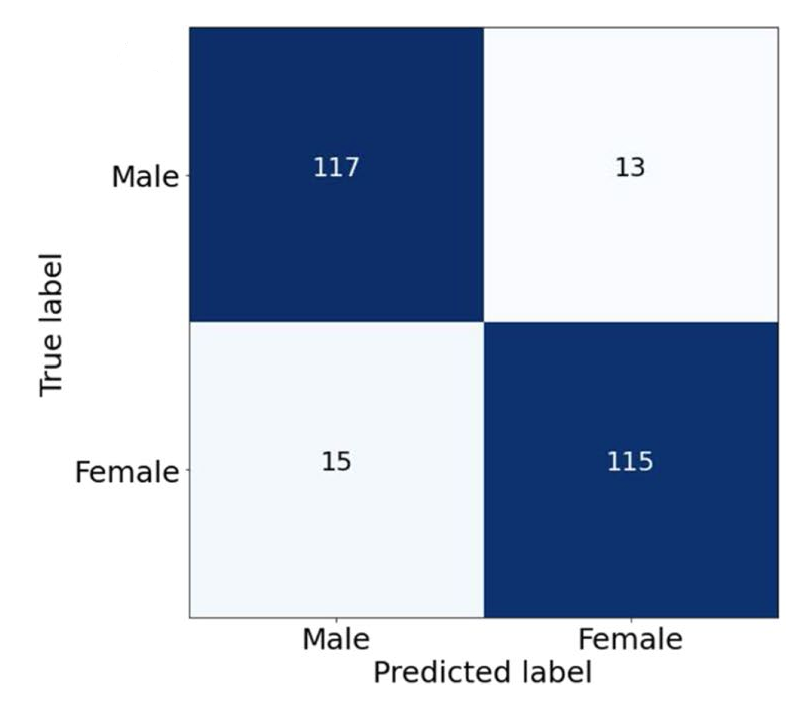
\includegraphics[width=0.6\textwidth]{capitulos/cap_02/imagenes/confusion_matrix_binary.png}
        \caption{
            Matriz de confusión para la estimación de sexo según el modelo \textit{random forest} 
            propuesto en \cite{bidmos2023}.
        } 
        \label{fig:conf_matrix_binary}
    \end{figure}
    
    \begin{figure}[h]
        \centering
    
        \begin{subfigure}[b]{0.3\textwidth}
            \centering
            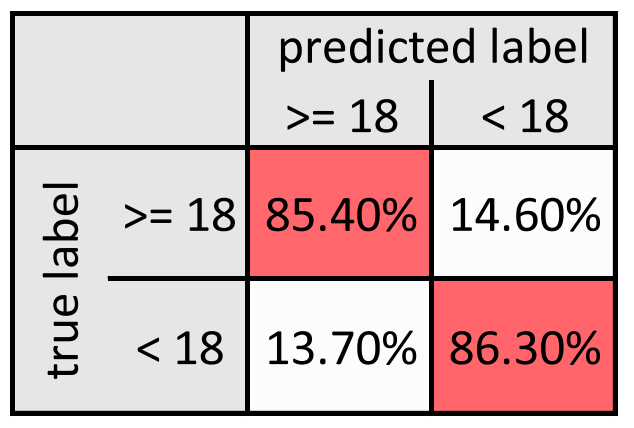
\includegraphics[width=\textwidth]{capitulos/cap_02/imagenes/confusion_matrix_binary_1.png}
            \caption{Sin información de sexo}
            \label{fig:conf_matrix_general}
        \end{subfigure}
        \hfill
        \begin{subfigure}[b]{0.3\textwidth}
            \centering
            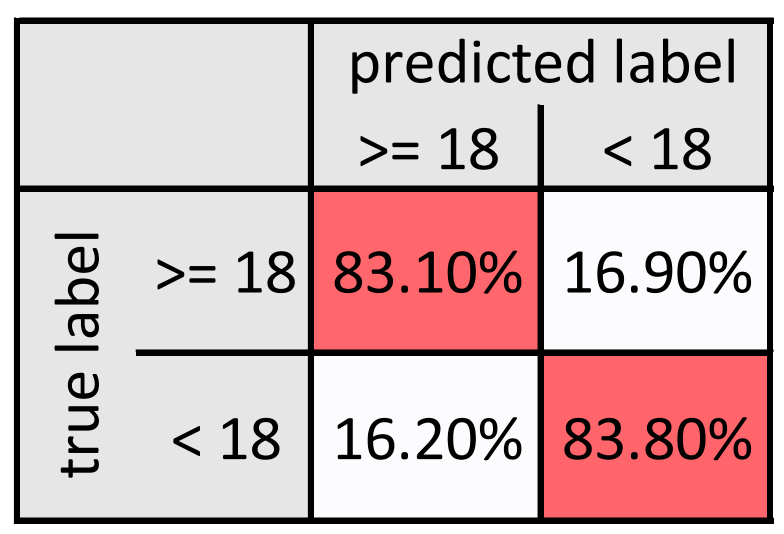
\includegraphics[width=\textwidth]{capitulos/cap_02/imagenes/confusion_matrix_binary_2.png}
            \caption{Sexo femenino}
            \label{fig:conf_matrix_female}
        \end{subfigure}
        \hfill
        \begin{subfigure}[b]{0.3\textwidth}
            \centering
            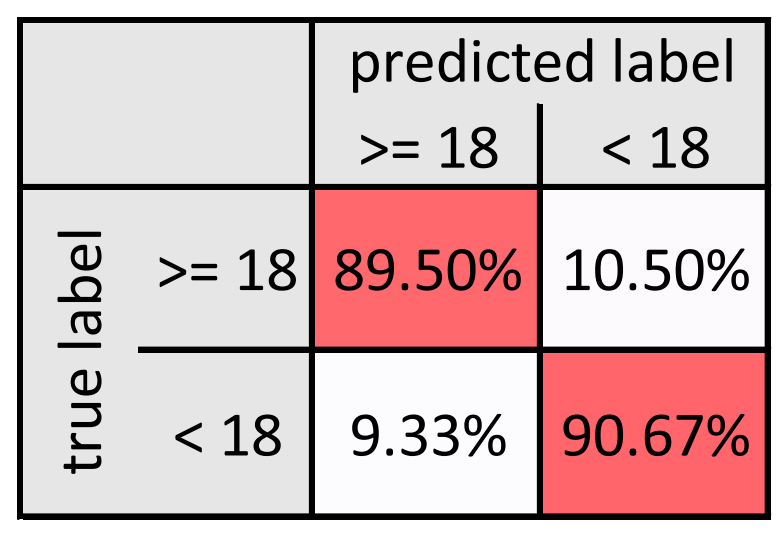
\includegraphics[width=\textwidth]{capitulos/cap_02/imagenes/confusion_matrix_binary_3.png}
            \caption{Sexo masculino}
            \label{fig:conf_matrix_male}
        \end{subfigure}
    
        \caption[
            Matrices de confusión para la estimación de mayoría/minoría de edad según el modelo de 
            \cite{porto2020}.
        ]{
            Matrices de confusión para la estimación de mayoría/minoría de edad según el modelo de 
            \cite{porto2020}.
            Se representan los valores de cada celda en términos porcentuales de los ejemplos reales que hay 
            de cada clase ($< 18$ y $\ge 18$), lo que permite comparar la matriz de confusión general de todos 
            los ejemplos (\ref{sub@fig:conf_matrix_general}) con la de ejemplos se sexo femenino 
            (\ref{sub@fig:conf_matrix_female}) y sexo masculino (\ref{sub@fig:conf_matrix_male}), permitiendo 
            identificar posibles sesgos en el modelo respecto al género, y así realizar una evaluación más 
            precisa del rendimiento del modelo en diferentes subgrupos de la población.
        }
        \label{fig:conf_matrix_binary_relative}

    \end{figure}


    \item La \textbf{cobertura empírica (\textit{empirical coverage}, EC)}, de forma análoga a la regresión, 
    mide la proporción de veces que la etiqueta verdadera está contenida dentro del conjunto predicho.

    $$
    EC = \frac{1}{n} \sum_{i=1}^{n} \mathbb{I}(y_i \in \Gamma_\alpha(x_i))
    $$

    \item El \textbf{tamaño del conjunto promedio (\textit{mean set size}, MSS)} mide qué cuántas etiquetas,
    en promedio, incluyen los conjuntos de predicción $\Gamma_\alpha(x)$.

    $$
    MSS = \frac{1}{n} \sum_{i=1}^n | \Gamma_\alpha(x_i) |
    $$

\end{itemize}


% ------------------------------------------------------------------------------------------------------------
% ------------------------------------------------------------------------------------------------------------

\section{Resultados}

\subsection{Estimación de edad}




\begin{figure}[h]
    \centering
    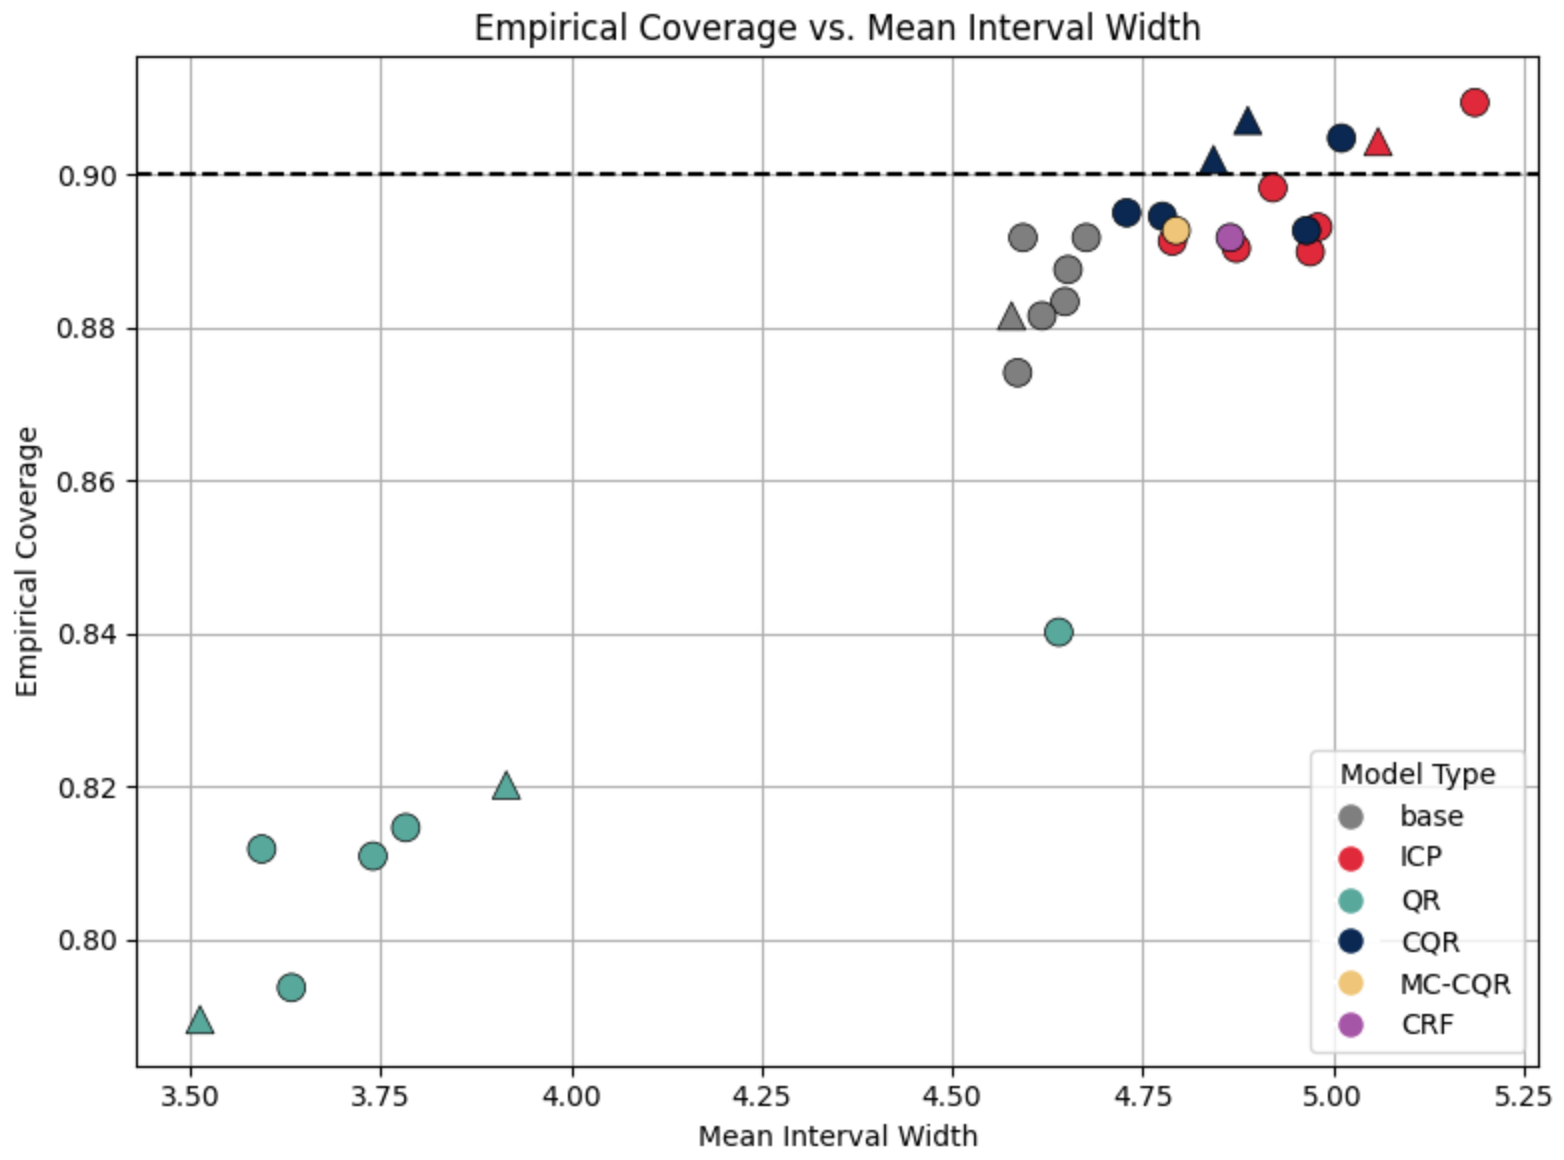
\includegraphics[width=\textwidth]{capitulos/cap_05/imagenes/EC-MIW.png}
    \caption[
        Gráfica de dispersión EC-MIW
    ]{
        Gráfica de dispersión EC-MIW. Triángulo = con sex embedding. 
    }
    \label{fig:ec-miw}
\end{figure}


\begin{figure}[h]
    \centering
    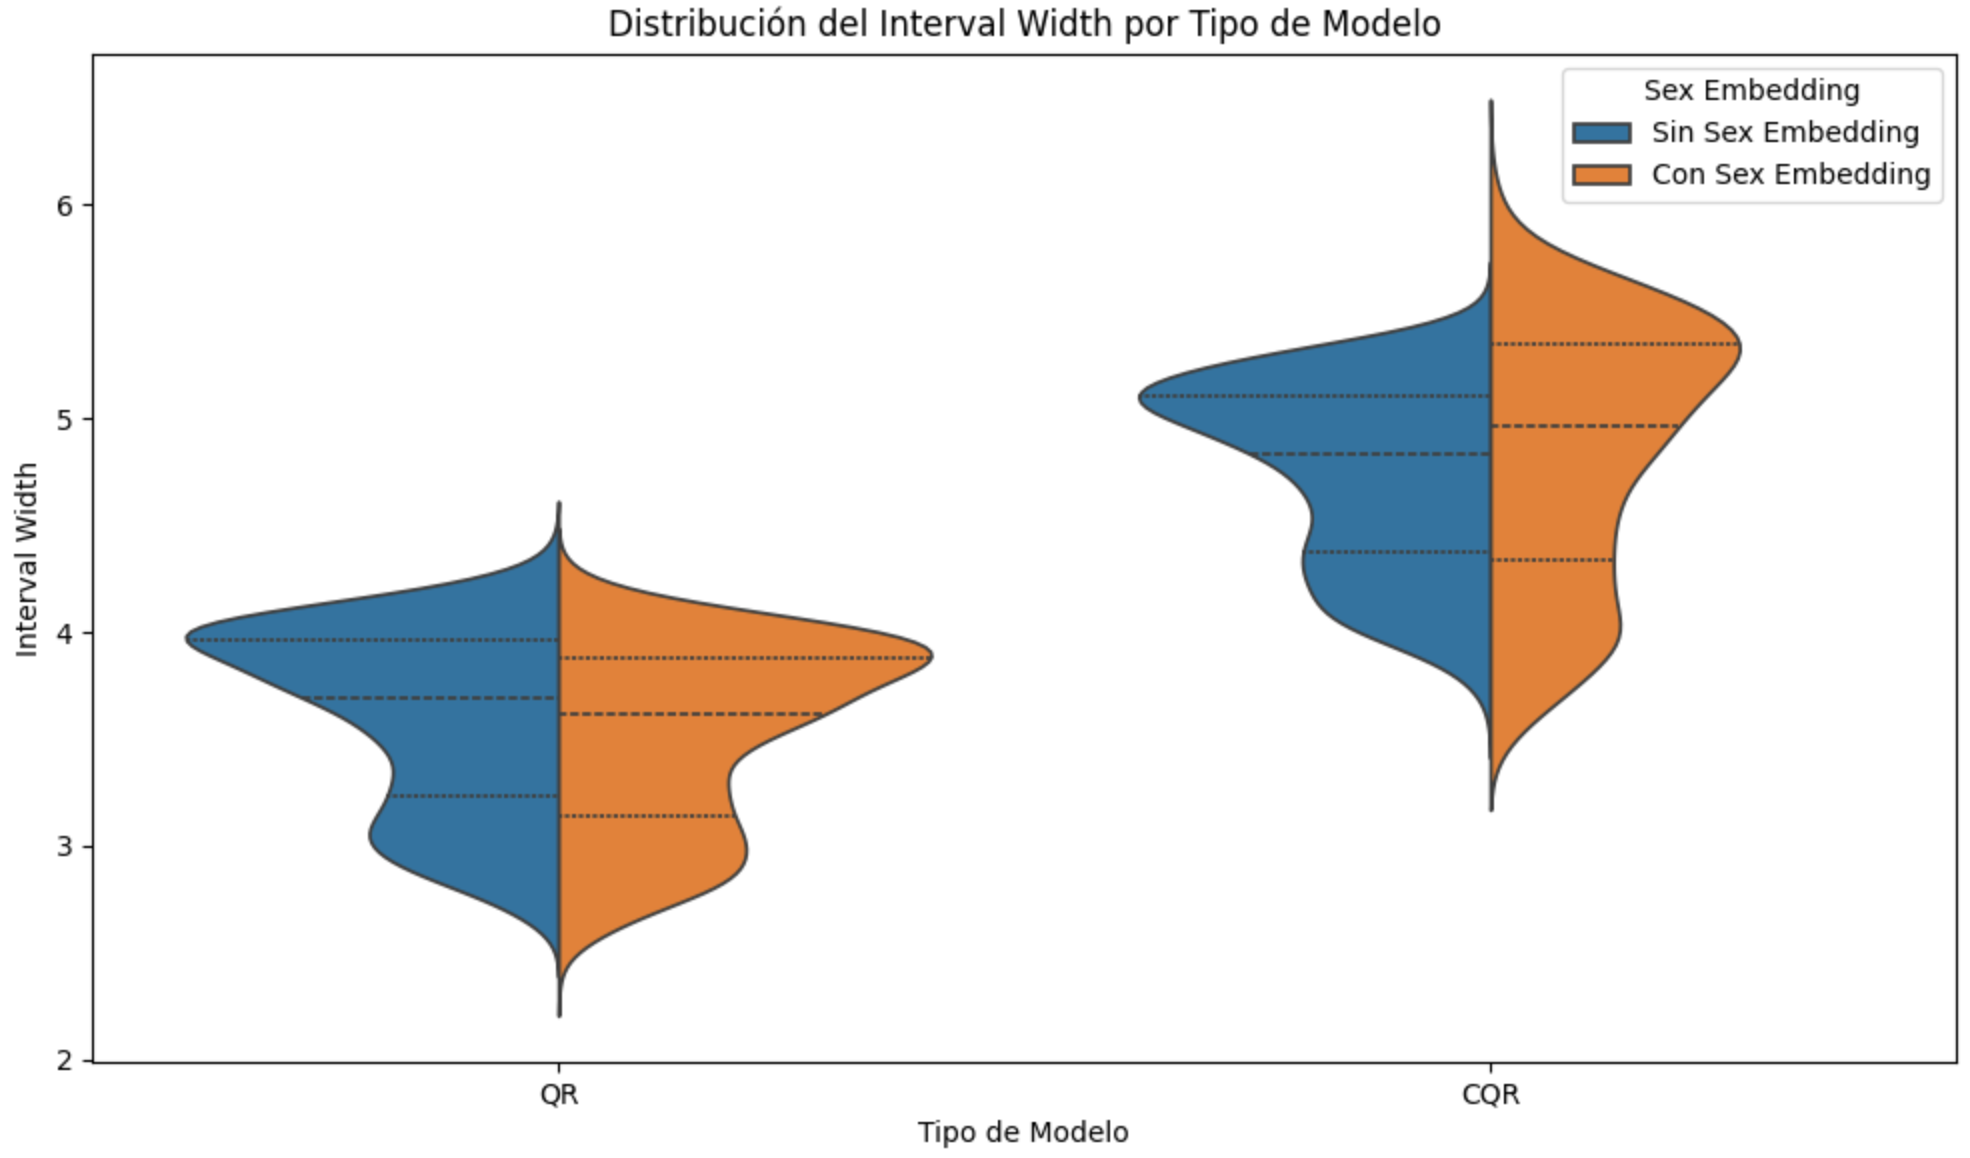
\includegraphics[width=\textwidth]{capitulos/cap_05/imagenes/violin_interval_width.png}
    \caption[
        Gráfica de violin de tamaños de intervalos
    ]{
        Gráfica de violin de tamaños de intervalos.
        Con estas diferencias entre problema con sex embedding y sin sex embedding, no sé si merece la pena
        esta comparación. Mi idea era que con sex embedding se reduciría la incertidumbre del problema y los 
        intervalos quedarías más ajustados, pero el rendimiento del modelo no mejora, y tampoco lo hacen por 
        consiguiente los intervalos de la CP. 
    }
    \label{fig:violin_interval_width}
\end{figure}


\begin{figure}[h]
    \centering
    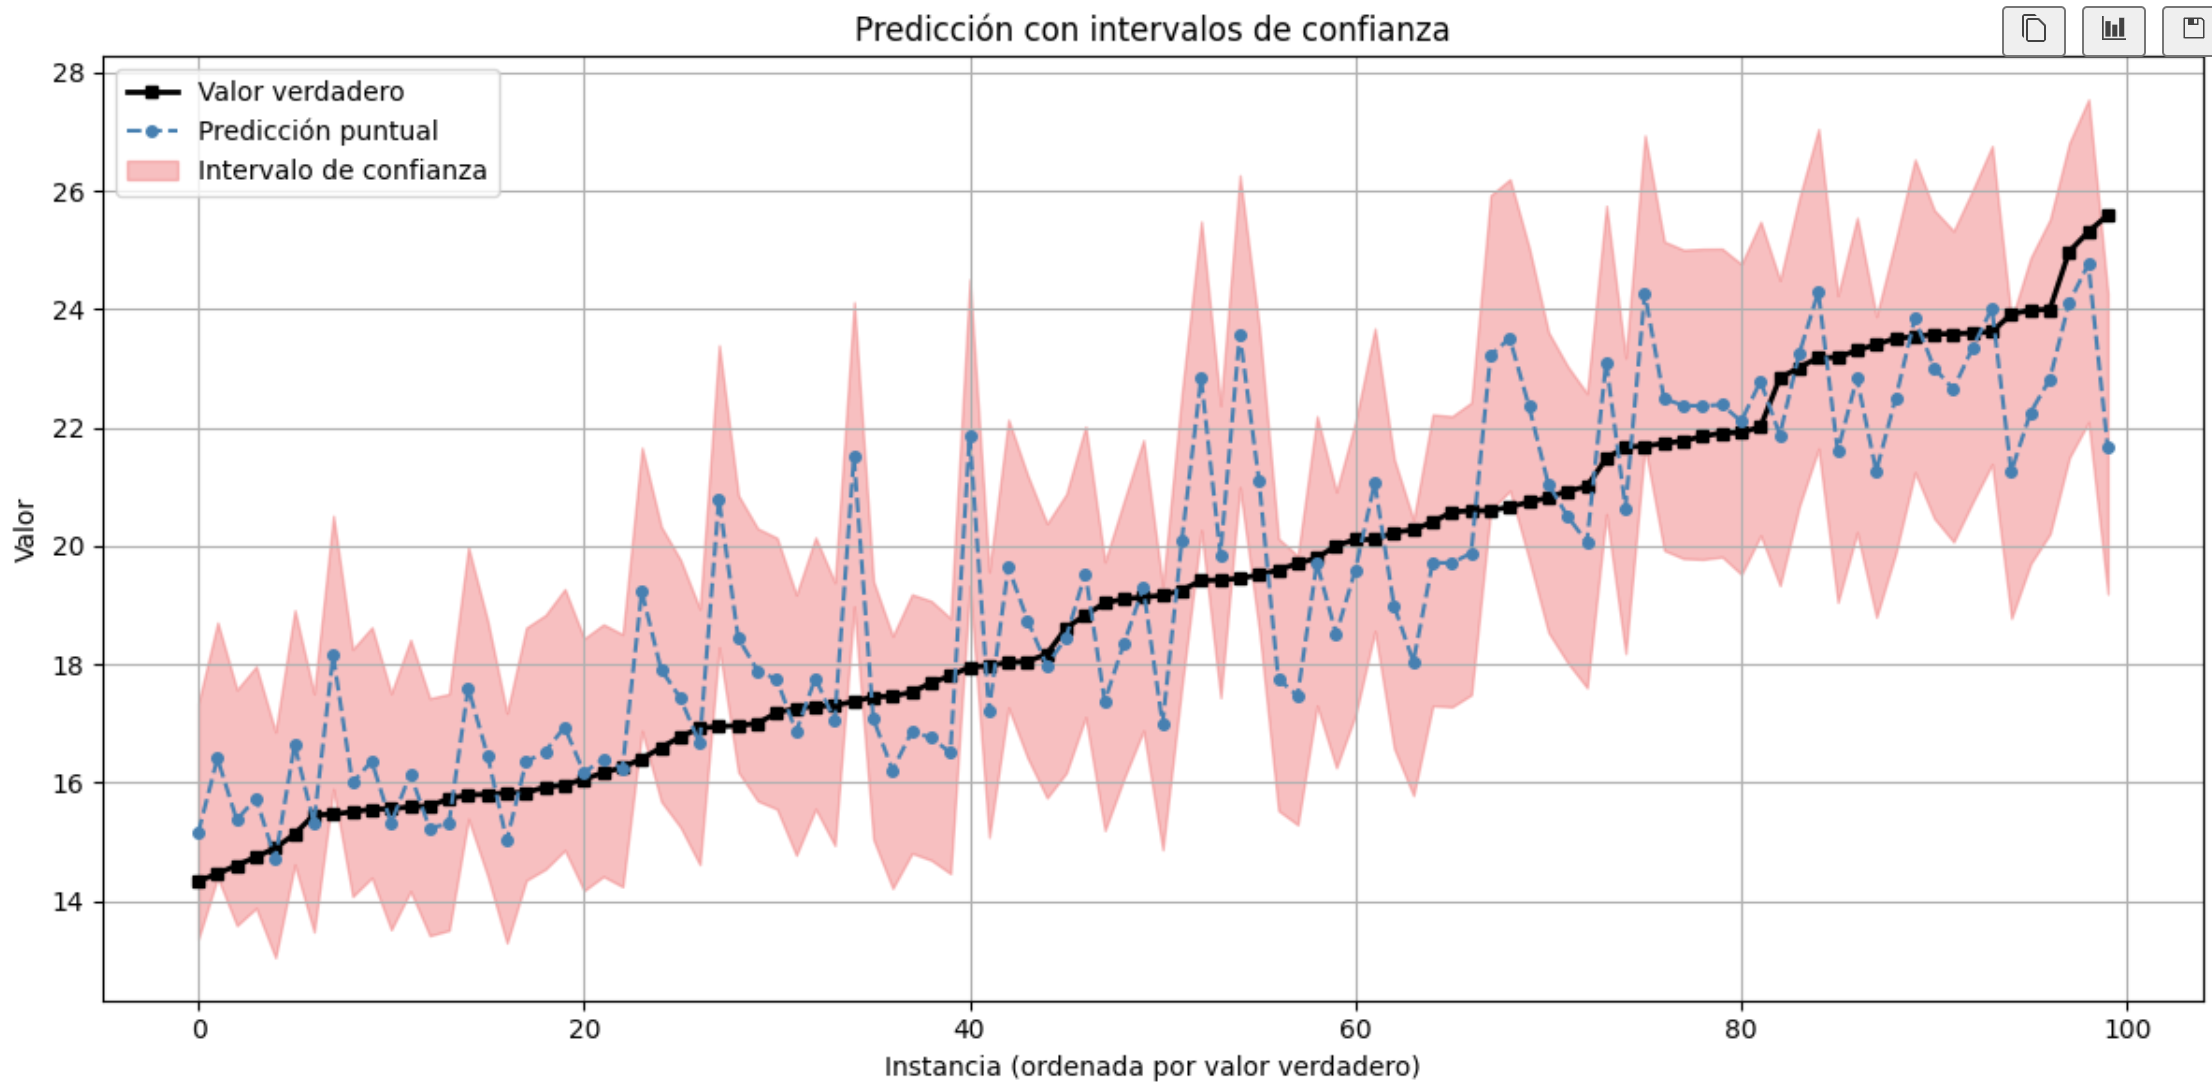
\includegraphics[width=\textwidth]{capitulos/cap_05/imagenes/conformal_prediction_sorted_by_true.png}
    \caption[
        Gráfica de líneas con predicción central e intervalo predictivo ordenado por valor real
    ]{
        Gráfica de líneas con predicción central e intervalo predictivo ordenado por valor real
    }
    \label{fig:conformal_prediction_sorted_by_true}
\end{figure}

\todo{Mejorar el diseño y legibilidad de todas las gráficas (JULIO)}

% ------------------------------------------------------------------------------------------------------------


Las mejoras de MCM sobre LAC no destacan en este problema donde las clases están balanceadas. 


% ------------------------------------------------------------------------------------------------------------




% ------------------------------------------------------------------------------------------------------------
% ------------------------------------------------------------------------------------------------------------


